%!TEX root = ../../Paper.tex

\chapter{Theoretical Background}
\label{cha:background}

\section{Big Data}
\label{sec:big-data}
The term \textit{Big Data} describes an enormous amount of data, which cannot be stored, managed or analyzed with conventional database tools \cite{web2011linkeddata}. Big Data can include different types of data, such as enterprise, machine-generated, sensor or social data \cite[3]{oraclebigdata}.

In the last few years, the analysis of Big Data became an essential aspect for many companies. Big social data analysis enables these companies to get more information about their customers' sentiment, satisfaction or opinion by collecting and analyzing data from social media services \cite{oraclebigdata}.

\section{Social Media}
\label{sec:social-media}
The term \textit{Social Media} belongs to web applications such as \enquote{social networks, blogs, multimedia content sharing sites and wikis} \cite{eu2013socialmedia}. Social networks such as Facebook, Twitter or Google+ are used by an increasing number of people. In September 2013, 73\% of online participants used at least one social networking site, of those 71\% were active on Facebook and about 19\% on Twitter \cite{pewresearchsocialmediafact}. Twitter, a popular microblogging service with over 284 million active monthly users\footnote{\url{http://about.twitter.com/company} \accessednote \label{aboutwitter}}, allows anyone to instantly post 140-characters text messages. Thereby, up to 500 million public Tweets are generated per day in more than 35 languages about nearly any imaginable topic\footref{aboutwitter}.  Social media applications enable people to connect with others as well as to publish content such as their interests, opinions, knowledge and ideas. During the past several years, user-generated-content has become more and more popular, which means that the users participating more in content creation, rather than just content consumption \cite[1]{Agichtein:2008:FHC:1341531.1341557}.  This behavior leads to an continuously increasing amount of unstructured social data and makes it impossible for humans to read through and analyze this immense amount of unstructured data. Therefore, advanced data mining and analysis techniques are necessary.

The traditional approach to gain insights into society, human beings and social relations required \enquote{questioning a large number of people about their feelings} \cite[1]{flaounas2012big}. In contrast, social media applications can provide those valuable information about the public \enquote{due to the fact that people use them to express their feelings} \cite[1]{flaounas2012big}. For instance, Twitter attracted many professionals to collect and analyze Tweets to gain valuable insights on anything from stock market to natural disasters by offering free API’s to access this huge amount of unstructured data.

\section{Data Analysis}
\label{sec:data-analysis}

\textbf{Machine learning} describes methods that enable computer systems to automatically learn from empirical data \cite{Domingos:2012:FUT:2347736.2347755,McKinsey2011}. Machine learning methods usually focus on the prediction and classification of information, based on training data that contains truthful information. A wide variety of applications exists for machine learning on big social data such as natural language processing, topic detection, text classification and sentiment analysis.

\vspace{10 mm}
\textbf{Data mining} is the process of finding valuable insights from large datasets. Therefore, data mining techniques try to extract meaningful patterns and associations in datasets by utilizing artificial intelligence, machine learning or statistical methods \cite{han2012mining}. In general, data mining is used as a synonym for the process of discovering knowledge from mostly unstructured data \cite[6\psqq]{han2012mining}.

\vspace{10 mm}
\textbf{Natural Language Processing (NLP)} is \enquote{a set of techniques [..] to analyze human language} \cite[29]{McKinsey2011}. Those techniques are often based on machine learning or statistical methods that enable computer systems to derive meaning from natural language. Therefore, NLP methods need to analyze and understand the syntax, semantics and the context of a sentence \cite{Linckels:2011:ESU:1995306}. Common application areas of NLP include stemming (described in chapter \ref{subsec:data-preparation}), named entity  recognition\footnote{Method to recognize well-known entities (e.g. person, location) in text.} and sentiment analysis.

\section{Trend Detection}
\label{sec:trends}
\textit{Trend detection} methods are used to detect emerging topics or trends by using Data Analysis methods. The keyword frequency approach is a popular method to discover trends in a big amount of unstructured text data \cite{journals/smarthome/Kim+13}. In the majority of cases, the input data is preprocessed to remove meaningless characters and words, as well as to prevent duplicated terms. After preprocessing the input data, the remaining words are ordered by their frequency of occurrence and the top $k$ words stand out as trending keywords \cite[213\psq]{journals/smarthome/Kim+13}.

Many social networks use hashtags to categorize social content, represent a topic or event and help users to discover certain content. A hashtag consists of \enquote{a sequence of non-whitespace characters preceded by the hash character} \cites[644]{conf/wsdm/TsurR12}[1427]{conf/asunam/ZhangWL13} (\eg{} \textit{\#NewYear} or \textit{\#AirAsia}). Hashtags are well suited for trend detection by measuring the number of uses in a certain time interval \cite[1427]{conf/asunam/ZhangWL13}. Using Trend Detection methods on social media content is an effective way to discover frequently used keywords and to show emerging topics in real-time \cite{journals/smarthome/Kim+13,TwitterDataAnalytics2013}.

A prominent example for large scale detection and prediction of trends based on huge amount of social data is \textit{Google Flu Trends}. Seasonal influenza, responsible for millions of illnesses and up to 500 thousand deaths per year, is known as a major health issue all over the world. An early detection of epidemics would reduce the significant effect of the pandemic and seasonal influenza. The project Google Flu Trends aims to monitor flu cases in real time based on various keywords with a strong correlation to the appearance and spread of seasonal flu to predict flu trends by analyzing social datasets \cites{Google09detection}[1]{Weber2014,Tech22014}. Figure \ref{fig:use_case_gft} visualizes the predicted flu activity in the United States in 2014.

\begin{figure}[H]
  \centering
        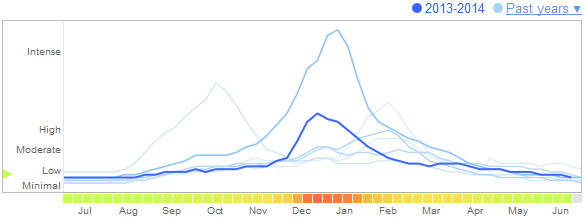
\includegraphics[width=30em]{gft_us}
  \caption[Flu activity in the United States]{Flu activity in the United States \cite{gft2014}}
  \label{fig:use_case_gft}
  \vspace{-1.3em}
\end{figure}